\begin{figure}
    \begin{center}
    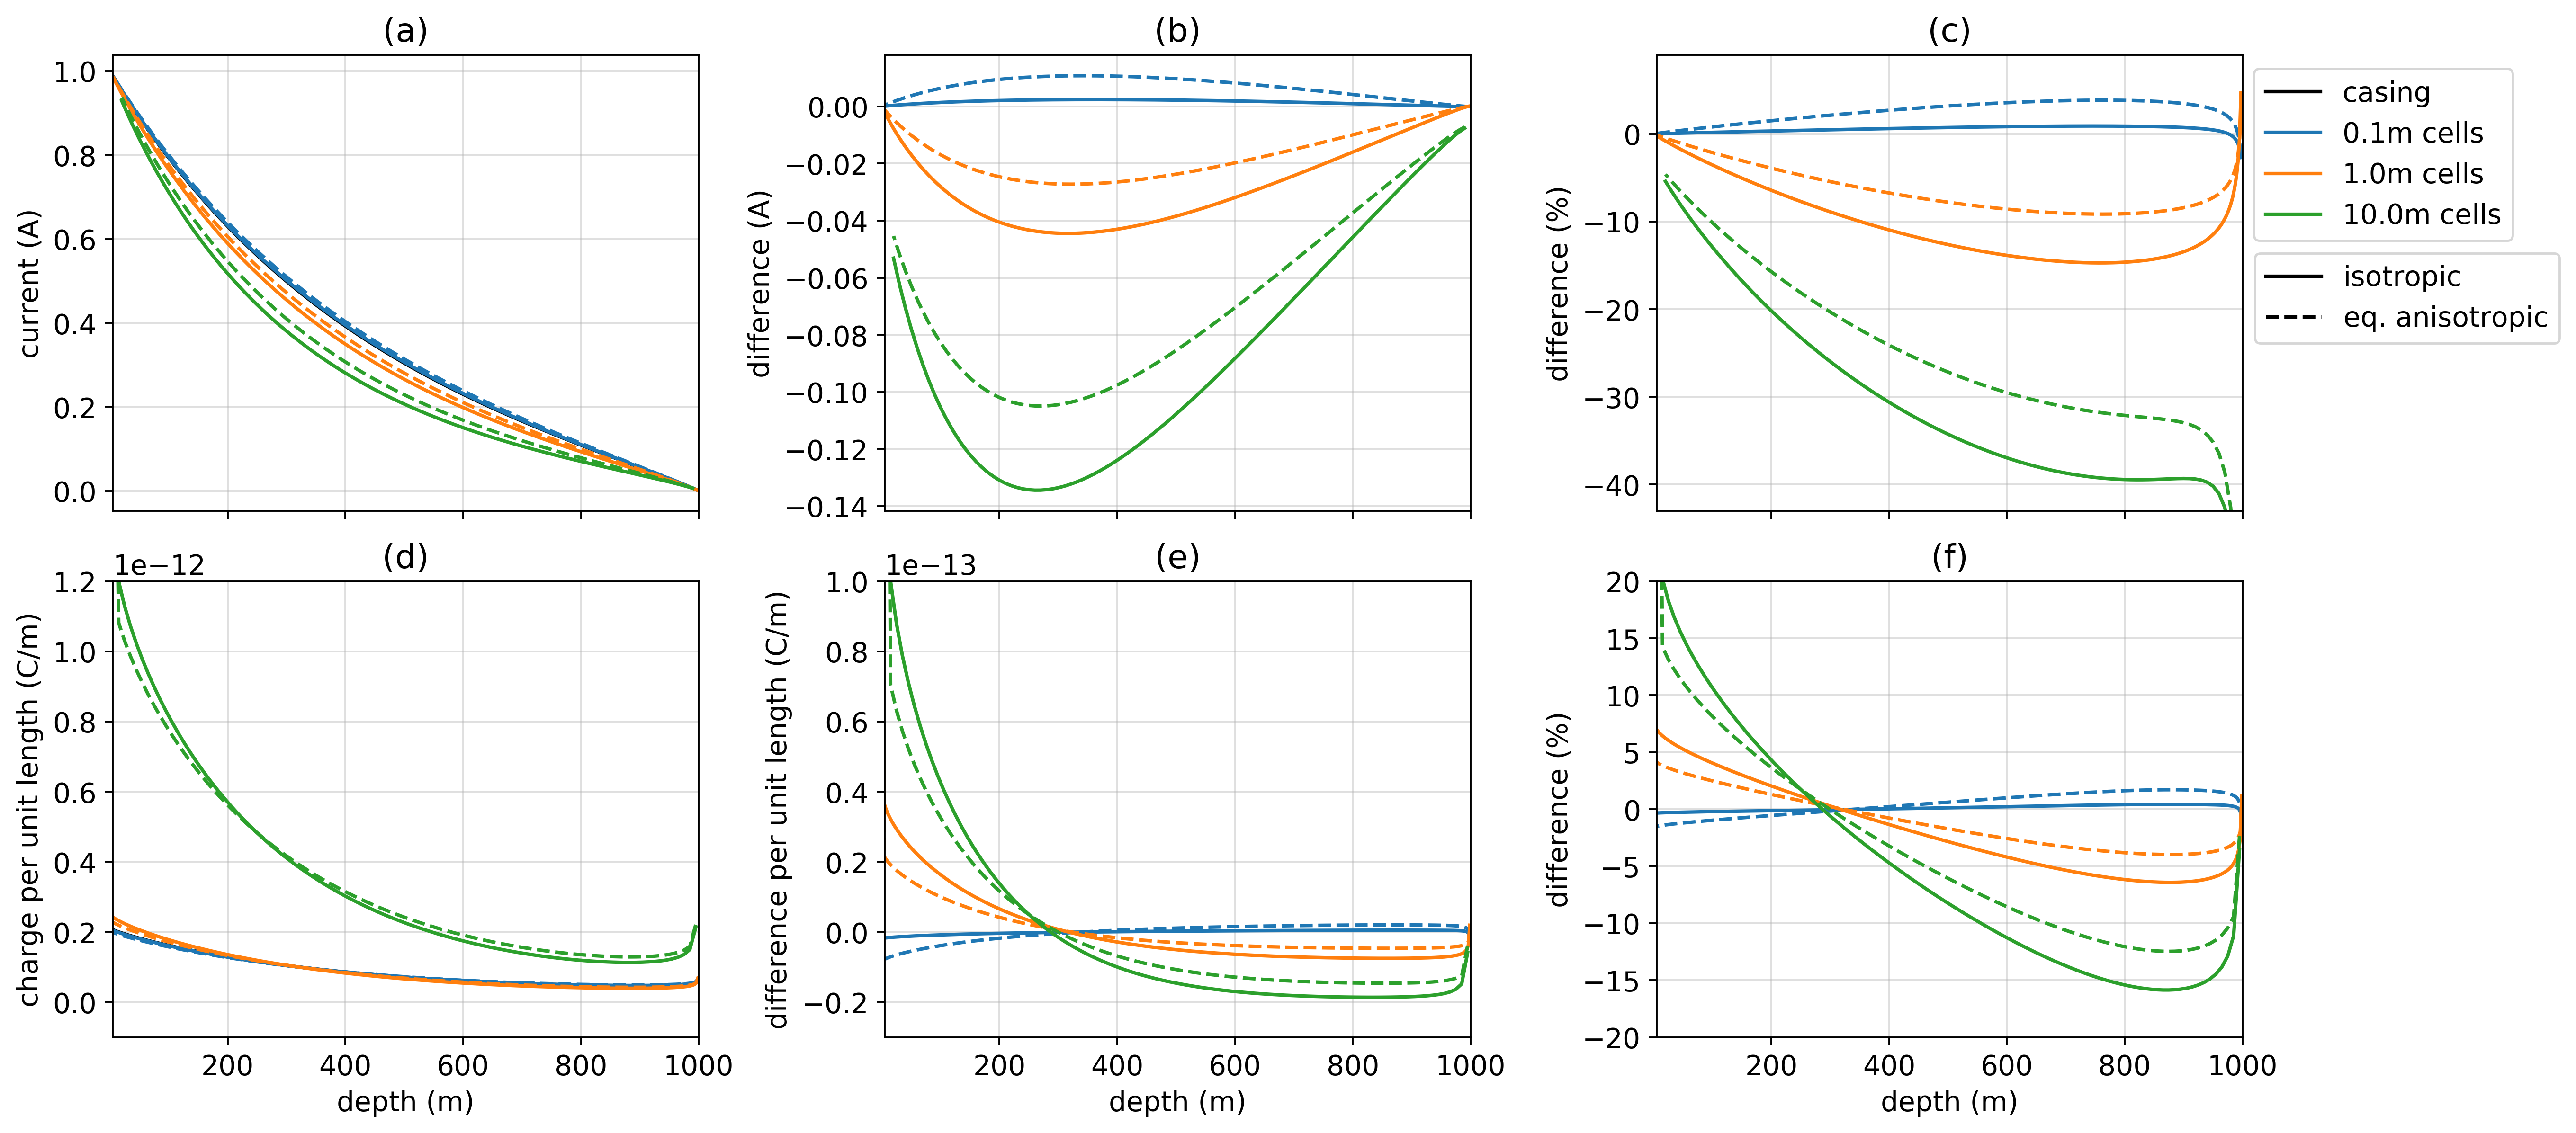
\includegraphics[width=\textwidth]{figures/approximating_wells_cartesian.png}
    \end{center}
\caption{
    Currents (top row) and charges (bottom row) along the length of
    a steel cased well represnted on a 3D cylindrical mesh which has
    4 cells radially across the width of the casing and 2.5m height (black line),
    a tensor mesh with 0.1m $\times$ 0.1m $\times$ 2.5m cells discretizing the casing (blue lines),
    a tensor mesh with 1m $\times$ 1m $\times$ 2.5m cells discretizing the casing (orange lines),
    and a tensor mesh with 10m $\times$ 10m $\times$ 10m cells discretizing the casing.
    The solid lines show simulations with an isotropic conductivity defined to preserve the
    product of the conductivity and cross-sectional area of the casing. The dashed lines
    use an anisotropic conductivity to represent the casing. The vertical component preserved the product
    of the conductivity and cross-sectional area of the casing while the horizontal components are an
    average of the resistivity and cross-sectional area of the casing and background
    (and equals the conductivity of the background, $0.1$ S/m, for both the 1m and 10m cells).
    In (a), we show the vertical current in the casing,
    (b) shows the difference from the true, hollow-cased well
    in the vertical current within the casing, and (c) shows that difference as a percentage
    of the true currents. In (d), we show the charge per unit length along the casing, (e)
    shows the difference from the true, hollow-cased well and (e) shows that differences as
    a percentage of the true charge distribution.
}
\label{fig:approximating_wells_cartesian}
\end{figure}
